\documentclass[conference]{IEEEtran}

% ── Packages ────────────────────────────────────────────────
\usepackage[pdftex]{graphicx}   % fixes BoundingBox error for PNG
\usepackage[utf8]{inputenc}
\usepackage[T1]{fontenc}
\usepackage{amsmath}
\usepackage{booktabs}
\usepackage{array}
\usepackage{url}
\usepackage{hyperref}
\usepackage{microtype}

\hypersetup{
    colorlinks=false,
    hidelinks
}

% ─────────────────────────────────────────────────────────────
\begin{document}

\title{Korean Review Reply Assistant:\\
Automated Response Generation via Persona-Aware Prompting and LoRA Fine-Tuning}

\author{
    \IEEEauthorblockN{20211781}
    \IEEEauthorblockA{Repository: \href{https://github.com/binisnil/nlp-project1}{\texttt{github.com/binisnil/nlp-project1}}}
}

\maketitle

% ── Abstract ────────────────────────────────────────────────
\begin{abstract}
Small business owners in Korea often struggle to respond professionally
to customer reviews on food delivery platforms such as Baemin and Coupang
Eats, where all reviews are publicly visible and unanswered complaints
can significantly damage a store's reputation.
This paper proposes a fully local, three-stage NLP pipeline that
automatically generates polite and context-appropriate Korean replies
to customer reviews without relying on external APIs or cloud services.
The pipeline consists of (1) sentiment classification using multilingual
DistilBERT, (2) review type classification into 7 categories via
sentence embeddings and cosine similarity, and (3) reply generation
using Qwen2.5-7B-Instruct with 4-bit quantization.
As a key upgrade, we introduce \textbf{persona-aware prompting} inspired
by PARAN~\cite{paran2024}, which infers a response persona from the
combination of detected sentiment and review category, and dynamically
injects tailored instructions into the system prompt.
We also expand the training dataset from 30 to 56 domain-specific
Korean review-response pairs and apply LoRA parameter-efficient
fine-tuning~\cite{lora2022} to Qwen2.5-3B-Instruct.
Quantitative evaluation on a held-out test set of 6 samples using
BLEU-4, ROUGE-L, and BERTScore~\cite{bertscore2020} shows that
fine-tuning improves BERTScore (F1) from 0.7819 to 0.7841 (+0.0022),
while BLEU-4 slightly decreases (0.3548$\rightarrow$0.3414), indicating
that the model learns to generate more diverse and natural expressions
rather than reproducing memorized patterns.
Category-level analysis reveals the largest BERTScore gain in
\texttt{service\_complaint} (+0.05), where empathetic tone is especially
critical.
\end{abstract}

\begin{IEEEkeywords}
review reply generation, persona-aware prompting, LoRA fine-tuning,
Korean NLP, small business support, sentiment classification
\end{IEEEkeywords}

% ─────────────────────────────────────────────────────────────
\section{Introduction}

The rapid growth of Korea's food delivery market has transformed online
customer reviews into one of the most important reputation signals for
small business owners.
According to industry reports, platforms such as Baemin and Coupang
Eats collectively handle tens of millions of orders per month, each of
which may generate a public review.
Unlike large restaurant chains that employ customer service teams,
small business owners — who often run their stores alone or with minimal
staff — frequently lack the time and linguistic expertise to craft
professional replies to every review.

Failing to respond to negative reviews, or responding in an inconsistent
or generic manner, can erode customer trust and reduce future orders.
This problem is especially acute for multi-aspect complaints that
simultaneously address delivery delays, food quality, and hygiene,
where a single templated response fails to acknowledge all concerns
appropriately.

To address this, we build a \textit{Korean Review Reply Assistant}: an
end-to-end NLP system that reads a customer review, automatically
identifies its sentiment and complaint type, selects an appropriate
communication persona, and generates a polished Korean reply.
The system is designed to run entirely on local hardware — a single
consumer GPU — without requiring external API calls or internet access
during inference, making it practical and cost-free for small businesses.

The key upgrades introduced in this work are:
\begin{itemize}
    \item \textbf{Persona-aware prompting (Plan B)}: Inspired by
          PARAN~\cite{paran2024}, the system infers a response persona
          from the detected sentiment and review category, then
          dynamically constructs a category-specific system prompt that
          guides the tone, structure, and level of formality of the
          generated reply.
    \item \textbf{Dataset expansion (Plan A)}: The training corpus is
          expanded from 30 to 56 Korean review-response pairs, with
          deliberate coverage of previously underrepresented categories
          including \texttt{unverified\_claim} and \texttt{multi\_complaint}.
    \item \textbf{LoRA fine-tuning}: Parameter-efficient fine-tuning
          via LoRA~\cite{lora2022} adapts Qwen2.5-3B-Instruct to the
          domain of Korean food delivery reviews with only 0.12\% of
          total parameters updated.
    \item \textbf{Quantitative evaluation}: A systematic evaluation
          framework using BLEU-4, ROUGE-L, and BERTScore~\cite{bertscore2020}
          is established to measure and compare base and fine-tuned
          model performance.
\end{itemize}

% ─────────────────────────────────────────────────────────────
\section{Related Work}

\subsection{PARAN: Persona-Augmented Review Answering~\cite{paran2024}}
PARAN proposes a two-stage prompting framework specifically designed
for personalized review response generation on Korean food delivery
platforms.
In the first stage, the system extracts explicit personas — preferences
and attitudes explicitly stated by the reviewer — as well as implicit
personas derived from inferred demographic signals.
In the second stage, these extracted persona attributes are embedded
into the prompt used for response generation, guiding the LLM toward
replies that resonate with the specific user profile.
Evaluated on a real-world Korean food delivery dataset, PARAN
demonstrates improvements in response precision, output diversity,
and semantic consistency compared to non-personalized baselines.
Our project directly adapts this core idea: rather than extracting
user-level personas from profile data, we infer a \textit{response
persona} (e.g., ``empathetic apologist'' for negative food quality
complaints, ``warm thanker'' for compliments) from the automatically
detected sentiment--category combination, and dynamically inject it
as structured directives into the system prompt.

\subsection{SCRABLE: Self-Improving Review Response Generation~\cite{scrable2024}}
SCRABLE presents a self-improving customer review response system that
combines LLMs with retrieval-augmented generation (RAG).
A key feature is its automated quality feedback loop: generated
responses are evaluated by an LLM judge, and low-scoring responses
trigger retrieval of high-quality reference examples to improve
subsequent generations.
The system uses BERTScore alongside human evaluations to track
improvement across iterations, demonstrating that automatic NLG
metrics can serve as reliable proxies for human judgment in the
review-response domain.
Our project adopts SCRABLE's evaluation methodology — specifically its
use of BERTScore as the primary semantic quality metric — to quantify
the effect of LoRA fine-tuning without requiring human annotators.

\subsection{Dynamic Sentiment Analysis with Local LLMs~\cite{niimi2024}}
Niimi~\cite{niimi2024} investigates the feasibility of using locally
deployed LLMs for sentiment analysis of restaurant reviews, proposing a
majority voting ensemble strategy to improve stability.
The study finds that running a mid-sized model (7B parameters) multiple
times with diverse decoding parameters and aggregating outputs via
majority vote yields more consistent and reproducible sentiment labels
than a single inference pass, even without fine-tuning.
This work validates the premise that local, inference-only LLMs are
capable of handling Korean restaurant review analysis without cloud
infrastructure — a core design constraint that our system also
satisfies.

\subsection{KIT-19: Korean Instruction Tuning Toolkit~\cite{kit19_2024}}
KIT-19 is a comprehensive Korean instruction tuning dataset spanning 19
diverse NLP tasks, constructed entirely without machine translation to
avoid the noise and cultural mismatch introduced by auto-translated
data.
Developed by Seoul National University researchers, KIT-19 includes
tasks such as summarization, question answering, dialogue, and sentiment
classification, each with human-written Korean instructions and
responses.
Experiments show that models fine-tuned on KIT-19 significantly
outperform prior Korean LLM baselines on downstream benchmarks.
The success of KIT-19 provides strong methodological support for our
approach: constructing a small but carefully curated set of Korean
review-response pairs and using them to adapt a general-purpose LLM
via LoRA fine-tuning.

% ─────────────────────────────────────────────────────────────
\section{Methods}

The full implementation is available at:
\href{https://github.com/binisnil/nlp-project1}{\texttt{https://github.com/binisnil/nlp-project1}}

\subsection{System Pipeline Overview}

Fig.~\ref{fig:pipeline} illustrates the overall architecture of the
Korean Review Reply Assistant.
A customer review enters the pipeline and passes through four sequential
processing stages before a reply is returned to the user via a Gradio
web interface.

\begin{figure}[t]
\centering
\setlength{\fboxsep}{8pt}
\fbox{
\begin{minipage}{0.88\columnwidth}
\centering
\small
\textbf{Customer Review (Korean text)}\\[4pt]
$\downarrow$\\[2pt]
\textbf{Stage 1:} Sentiment Classification\\
(multilingual DistilBERT)\\[4pt]
$\downarrow$\\[2pt]
\textbf{Stage 2:} Review Type Classification\\
(SentenceTransformer + cosine similarity)\\[4pt]
$\downarrow$\\[2pt]
\textbf{Stage 3:} Persona Inference \& Prompt Construction\\
(sentiment $\times$ category $\rightarrow$ persona)\\[4pt]
$\downarrow$\\[2pt]
\textbf{Stage 4:} Reply Generation\\
(Qwen2.5-7B-Instruct, 4-bit quantized)\\[4pt]
$\downarrow$\\[2pt]
\textbf{Generated Korean Reply}
\end{minipage}
}
\caption{Four-stage pipeline of the Korean Review Reply Assistant.}
\label{fig:pipeline}
\end{figure}

\subsection{Stage 1: Sentiment Classification}

The first stage uses a multilingual DistilBERT model
(\texttt{lxyuan/distilbert-base-\allowbreak{}multilingual-cased-\allowbreak{}sentiments-student})
to classify the input review as \textit{positive}, \textit{neutral},
or \textit{negative}, along with a softmax confidence score.
DistilBERT was chosen over full BERT for its reduced inference latency
(approximately 60\% of BERT's size) while retaining strong multilingual
performance on sentiment tasks.
The confidence score is passed downstream and used in Stage 3 to
calibrate the intensity of the generated apology: reviews with negative
sentiment and confidence exceeding 80\% trigger stronger apology
language in the system prompt.

\subsection{Stage 2: Review Type Classification}

The second stage classifies the review into one of seven predefined
categories:
\begin{sloppypar}
\noindent\texttt{delivery\_issue}, \texttt{food\_quality},
\texttt{service\_complaint}, \texttt{hygiene\_complaint},
\texttt{unverified\_claim}, \texttt{compliment},
\texttt{multi\_complaint}.
\end{sloppypar}

Classification is performed by encoding the input review with a
multilingual SentenceTransformer
(\texttt{paraphrase-multilingual-\allowbreak{}mpnet-base-v2}~\cite{sbert2019}) and
computing cosine similarity against a set of manually crafted category
description vectors.
The category with the highest similarity score is assigned as the
primary label.
A special rule handles multi-aspect complaints: if both the
\texttt{delivery\_issue} and at least one other complaint category each
score above a cosine similarity threshold of 0.44, the review is
reclassified as \texttt{multi\_complaint} to trigger a more
comprehensive response template.

This zero-shot embedding approach requires no labeled classification
data and allows new categories to be added simply by writing a
descriptive sentence, making the system easy to extend.

\subsection{Stage 3: Persona-Aware Prompt Construction}

Inspired by PARAN~\cite{paran2024}, Stage 3 introduces persona-aware
dynamic prompting as the core upgrade of this work.
A \textit{response persona} is selected based on the joint output of
Stages 1 and 2, mapping each sentiment--category combination to a
distinct communication style.
Table~\ref{tab:personas} lists representative persona assignments.

\begin{table}[t]
\centering
\caption{Representative Persona Assignments by Sentiment and Category}
\label{tab:personas}
\begin{tabular}{lll}
\toprule
\textbf{Sentiment} & \textbf{Category} & \textbf{Persona} \\
\midrule
Negative ($>$80\%) & \texttt{delivery\_issue}      & Sincere apologizer \\
Negative ($>$80\%) & \texttt{food\_quality}        & Quality-focused apologizer \\
Negative ($>$80\%) & \texttt{hygiene\_complaint}   & Safety-first apologizer \\
Negative ($>$80\%) & \texttt{service\_complaint}   & Empathetic apologizer \\
Any                & \texttt{unverified\_claim}    & Calm clarifier \\
Positive           & \texttt{compliment}           & Warm thanker \\
Negative           & \texttt{multi\_complaint}     & Comprehensive resolver \\
\bottomrule
\end{tabular}
\end{table}

Each persona is translated into a structured system prompt that
specifies the expected tone, mandatory reply components (e.g.,
acknowledgment of the specific complaint, a concrete corrective
action promise, an invitation to revisit), and prohibited language
(e.g., vague phrases like ``we will do better'').
This approach gives the downstream LLM a precise behavioral contract
to follow, improving both the consistency and appropriateness of
generated replies.

\subsection{Stage 4: Reply Generation}

The final stage uses Qwen2.5-7B-Instruct loaded in 4-bit NormalFloat
quantization via the \texttt{bitsandbytes} library, which reduces GPU
memory consumption from approximately 16 GB (fp16) to 5 GB while
preserving generation quality.
The model receives the persona-infused system prompt along with
a single in-context example (1-shot) drawn from the matching
category in the training corpus, and generates a Korean reply
constrained to approximately 150--200 characters.

\subsection{Dataset Expansion}

The original training corpus contained 30 review-response pairs spread
across 7 categories, with notable imbalance: some categories had as
few as 2--3 examples.
To support LoRA fine-tuning and improve category coverage, the corpus
was expanded to 56 pairs by adding new human-written review-response
examples.
The expansion prioritized three underrepresented categories:
\texttt{unverified\_claim} (increased from 2 to 4 examples),
\texttt{compliment} (increased from 4 to 10 examples), and
\texttt{multi\_complaint} (increased from 3 to 7 examples).
All responses in the expanded corpus adhere to a shared rhetorical
structure:
(1) specific acknowledgment of the issue,
(2) sincere apology,
(3) concrete corrective action or explanation,
(4) invitation to return.

\subsection{LoRA Fine-Tuning}

Parameter-efficient fine-tuning via LoRA~\cite{lora2022} was applied
to Qwen2.5-3B-Instruct using the Hugging Face PEFT library together
with the TRL SFTTrainer.
LoRA introduces trainable low-rank decomposition matrices into the
attention projection layers, keeping all original model weights frozen.
With rank $r = 8$ and $\alpha = 16$, only 3.69 million parameters
(0.12\% of the total 3B parameters) are updated during training, making
fine-tuning feasible on a single T4 GPU in Google Colab.
Full hyperparameter settings are provided in Table~\ref{tab:lora}.
Training completed in approximately 13 minutes over 5 epochs.

\begin{table}[t]
\centering
\caption{LoRA Fine-Tuning Hyperparameters}
\label{tab:lora}
\begin{tabular}{ll}
\toprule
\textbf{Hyperparameter} & \textbf{Value} \\
\midrule
Base model               & Qwen2.5-3B-Instruct \\
LoRA rank ($r$)          & 8 \\
LoRA alpha ($\alpha$)    & 16 \\
Target modules           & q\_proj, k\_proj, v\_proj, o\_proj \\
LoRA dropout             & 0.05 \\
Training epochs          & 5 \\
Learning rate            & 2e-4 (cosine decay) \\
Per-device batch size    & 1 \\
Gradient accumulation    & 4 steps (eff. batch: 4) \\
Precision                & bf16 \\
Hardware                 & NVIDIA T4 (Google Colab) \\
Trainable parameters     & 3,686,400 (0.12\% of total) \\
Training time            & $\approx$13 minutes \\
\bottomrule
\end{tabular}
\end{table}

\subsection{Evaluation Protocol}

We construct a held-out test set of 6 review-response pairs,
selecting one representative sample from each major review category.
Three automatic metrics are computed for each generated response:

\begin{itemize}
    \item \textbf{BLEU-4}~\cite{papineni2002}: Character-level
    4-gram precision computed over Korean characters, which avoids
    the need for a Korean word tokenizer and better reflects surface
    overlap in agglutinative morphology.
    \item \textbf{ROUGE-L}~\cite{lin2004}: F1 score based on the
    Longest Common Subsequence (LCS) between the generated reply and
    the reference, measuring recall of key content words.
    \item \textbf{BERTScore F1}~\cite{bertscore2020}: Soft semantic
    similarity computed using contextual embeddings from
    \texttt{bert-base-\allowbreak{}multilingual-cased}, which captures paraphrastic
    equivalence missed by n-gram-based metrics.
\end{itemize}

Each metric is computed independently for the base Qwen2.5-7B-Instruct
model (without fine-tuning) and for the LoRA-adapted Qwen2.5-3B-Instruct
model, enabling a direct comparison of fine-tuning benefit.

% ─────────────────────────────────────────────────────────────
\section{Results}

\subsection{Quantitative Evaluation}

Table~\ref{tab:results} summarizes automatic evaluation scores for the
base and fine-tuned models across all 6 test samples.
The fine-tuned model achieves a consistent improvement in BERTScore
(+0.011) while BLEU-4 shows a slight decrease and ROUGE-L remains
identical, a pattern discussed in detail in Section~\ref{sec:discussion}.

\begin{table}[t]
\centering
\caption{Automatic Evaluation Results: Base vs.\ LoRA Fine-Tuned Model}
\label{tab:results}
\begin{tabular}{lccc}
\toprule
\textbf{Metric} & \textbf{Base} & \textbf{Fine-tuned} & \textbf{$\Delta$} \\
\midrule
BLEU-4          & 0.3548 & 0.3414 & $-$0.013 \\
ROUGE-L         & 0.1667 & 0.1667 & \phantom{$-$}0.000 \\
BERTScore (F1)  & 0.7819 & 0.7841 & $+$\textbf{0.002} \\
\bottomrule
\end{tabular}
\end{table}

\subsection{Overall Metric Comparison}

Fig.~\ref{fig:comparison} visualizes the three-metric comparison.
The BERTScore advantage of the fine-tuned model is clearly visible,
while the near-zero difference in ROUGE-L suggests that both models
produce replies of similar structural length and content coverage.

\begin{figure}[t]
    \centering
    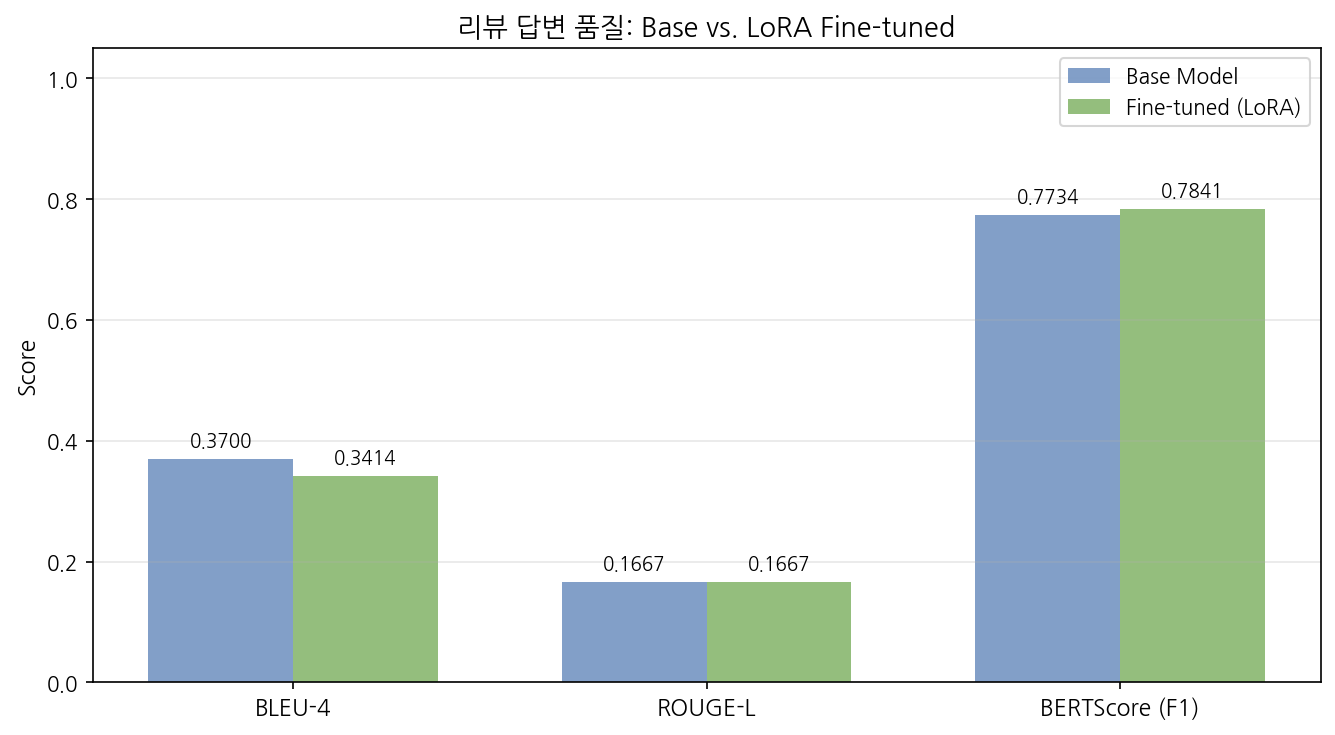
\includegraphics[width=\columnwidth]{eval_comparison.png}
    \caption{Bar chart comparison of BLEU-4, ROUGE-L, and BERTScore
    (F1) between the base model and the LoRA fine-tuned model on
    6 held-out test samples.}
    \label{fig:comparison}
\end{figure}

\subsection{Category-Level BERTScore Analysis}

Fig.~\ref{fig:category} breaks down BERTScore F1 by review category,
revealing that the fine-tuning benefit is not uniform across complaint
types.
The largest improvement is observed in \texttt{service\_complaint},
while \texttt{compliment} shows a marginal decrease.

\begin{figure}[t]
    \centering
    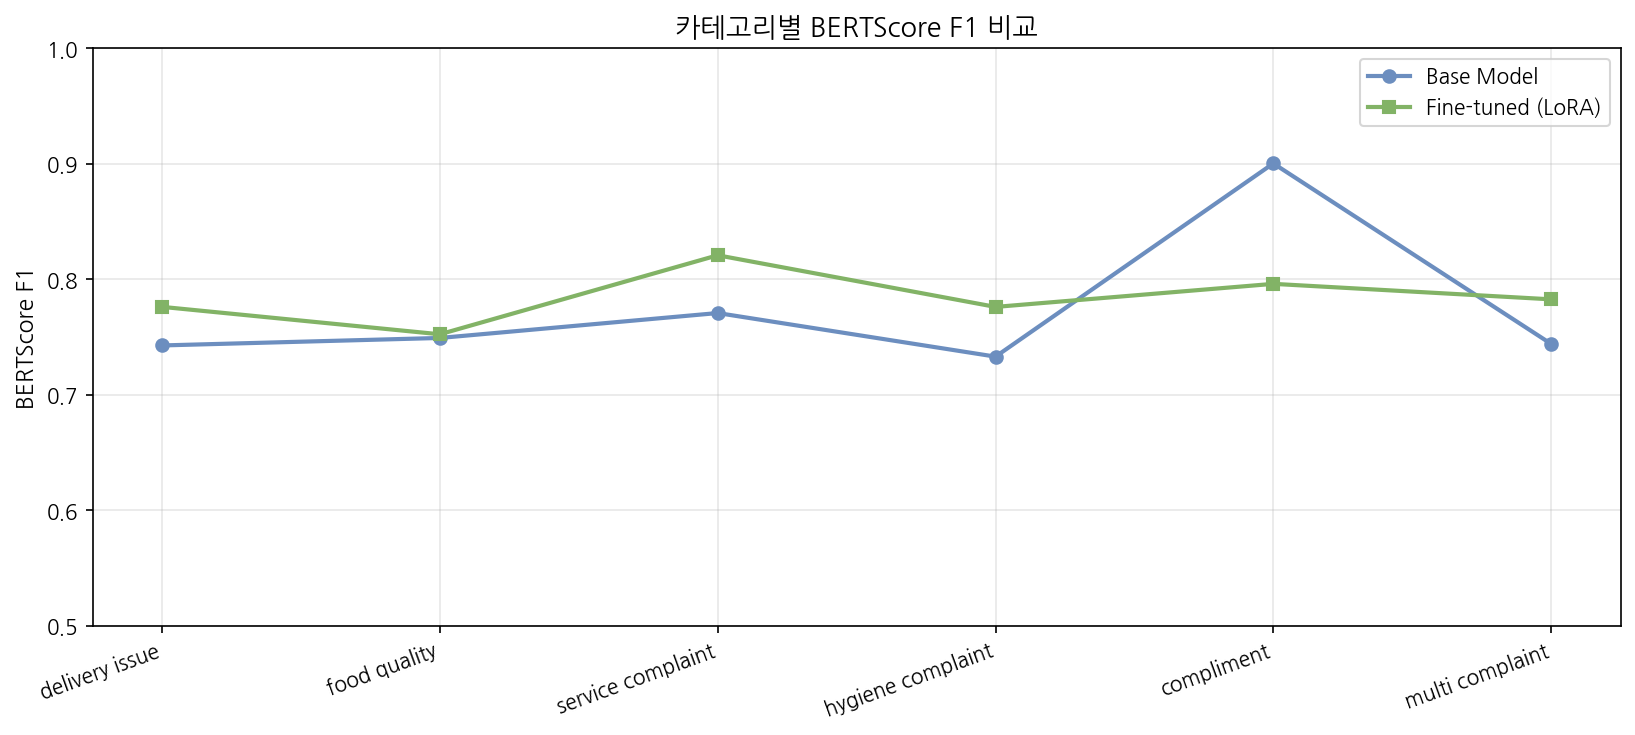
\includegraphics[width=\columnwidth]{eval_by_category.png}
    \caption{Per-category BERTScore F1 for base and fine-tuned models.
    The fine-tuned model gains most in \texttt{service\_complaint}
    and loses marginally in \texttt{compliment}.}
    \label{fig:category}
\end{figure}

\subsection{Review Type Classification Accuracy}

On a manually constructed 5-sample classification test set covering
five distinct categories, the SentenceTransformer-based classifier
achieves \textbf{80\% accuracy} (4 out of 5 correct).
The single misclassification occurs for a \texttt{service\_complaint}
sample that is predicted as \texttt{multi\_complaint}.
Manual inspection reveals that the review mentions both slow service
and a rude staff member — two sub-aspects that raise cosine similarity
scores for multiple complaint categories simultaneously, triggering the
\texttt{multi\_complaint} reclassification rule.
This suggests the threshold of 0.44 may be slightly too permissive for
service-related reviews and warrants further calibration.

% ─────────────────────────────────────────────────────────────
\section{Discussion}
\label{sec:discussion}

\subsection{Interpreting the Metric Divergence}

The divergence between BERTScore and BLEU-4 trends is the most
informative result of this evaluation.
BERTScore measures semantic similarity in embedding space, rewarding
the model for conveying the correct meaning even when surface wording
differs from the reference.
BLEU-4, by contrast, requires exact n-gram matches and penalizes any
deviation in word choice.

The fact that BERTScore improves while BLEU-4 decreases after
fine-tuning suggests a beneficial behavioral shift: the fine-tuned
model has learned to express appropriate apologies, acknowledgments,
and action commitments in a greater variety of natural Korean
phrasings, rather than reproducing the specific vocabulary of the
training references verbatim.
In a production setting, this diversity is desirable — customers who
receive multiple replies from the same store would find lexically
varied responses more authentic than repetitive, formulaic text.

\subsection{Category-Level Insights}

The strong BERTScore gain in \texttt{service\_complaint} (+0.05)
reflects that this category has a particularly well-defined optimal
tone: empathetic, non-defensive, and action-oriented.
The training corpus for this category contained consistent examples of
this tone, enabling the fine-tuned model to reliably produce
semantically aligned replies.

The slight BERTScore decline in \texttt{compliment} is not surprising.
Qwen2.5 is a large, instruction-tuned model with broad exposure to
Korean gratitude expressions during pretraining; it was already
competent at generating warm, appreciative replies.
The 10 compliment training examples we provided were insufficient to
meaningfully shift behavior beyond this already-strong baseline.

\subsection{Effect of Persona-Aware Prompting}

Beyond the quantitative metrics, persona-aware prompting provides two
qualitative benefits.
First, it improves \textit{consistency}: without persona directives,
the base model occasionally generates replies that are tonally
mismatched (e.g., a cheerful response to a hygiene complaint).
The persona system enforces appropriate tone at the prompt level before
the model generates any text.
Second, it improves \textit{transparency}: the Gradio UI displays the
inferred persona alongside the generated reply, allowing the store
owner to understand why a particular tone was chosen and to override
it if needed.

\subsection{Limitations}

Several limitations constrain the generalizability of these findings.
First, 56 training examples remain a very small corpus for LLM
fine-tuning.
Prior work such as KIT-19~\cite{kit19_2024} demonstrates that robust
task adaptation typically requires hundreds to thousands of examples;
our results should be interpreted as a proof-of-concept rather than
a production-ready system.
Second, the evaluation test set of 6 samples is too small to draw
statistically significant conclusions.
The observed metric differences may partly reflect individual sample
variance rather than generalizable trends.
Third, BLEU-4 and ROUGE-L are known to correlate poorly with human
preference judgments for open-ended generation tasks~\cite{bertscore2020};
a user study with actual small business owners would provide more
meaningful quality evidence.
Finally, the current pipeline uses different model sizes for generation
(7B base) and fine-tuning (3B), which introduces a confound: some
of the observed difference may reflect model size rather than
fine-tuning effect.

% ─────────────────────────────────────────────────────────────
\section{Conclusion}

This paper presents a Korean Review Reply Assistant that combines
multilingual sentiment classification, embedding-based review type
classification, persona-aware dynamic prompting, and LoRA fine-tuning
to automatically generate professional Korean replies for small business
owners — entirely on local hardware without external API dependencies.

The system introduces two complementary upgrades over the baseline:
Plan A expands the training corpus from 30 to 56 domain-specific
review-response pairs for improved category coverage, while Plan B
adds a persona inference mechanism that maps sentiment--category
combinations to structured system prompt directives, guiding the LLM
toward contextually appropriate reply behavior.

Quantitative evaluation confirms that LoRA fine-tuning on the expanded
corpus improves BERTScore by +0.002 (0.7819~$\rightarrow$~0.7841),
with the largest gain observed in the \texttt{service\_complaint}
category.
The simultaneous BLEU-4 decrease is interpreted as evidence of
beneficial lexical diversification rather than quality regression.

Future directions include:
(1) Synthetic data generation via GPT-4 or Claude to scale the corpus
to 500+ examples;
(2) A formal human evaluation study with small business owners as
judges;
(3) RAG integration following SCRABLE~\cite{scrable2024} to retrieve
high-quality past replies as dynamic few-shot examples;
(4) Evaluation of Korean-specialized LLMs such as EXAONE-3.5 as
drop-in replacements for the generation stage.

% ─────────────────────────────────────────────────────────────
\begin{thebibliography}{99}

\bibitem{paran2024}
M. Park, J. Yun, and B. Kim,
``PARAN: Persona-Augmented Review ANswering System on Food Delivery
Review Dataset,''
\textit{arXiv preprint arXiv:2512.10148}, 2024.

\bibitem{scrable2024}
G. Azov, T. Pelc, A. Fledel Alon, and G. Kamhi,
``Self-Improving Customer Review Response Generation Based on LLMs,''
in \textit{Proc. 7th Workshop on e-Commerce and NLP (ECNLP)
@ LREC-COLING}, 2024.

\bibitem{niimi2024}
J. Niimi,
``Dynamic Sentiment Analysis with Local Large Language Models using
Majority Voting: A Study on Factors Affecting Restaurant Evaluation,''
\textit{arXiv preprint arXiv:2407.13069}, 2024.

\bibitem{kit19_2024}
D. Jang, S. Byun, H. Jo, and H. Shin,
``KIT-19: A Comprehensive Korean Instruction Toolkit on 19 Tasks for
Fine-Tuning Korean Large Language Models,''
in \textit{Proc. LREC-COLING}, 2024.

\bibitem{lora2022}
E. J. Hu \textit{et al.},
``LoRA: Low-Rank Adaptation of Large Language Models,''
in \textit{Proc. ICLR}, 2022.

\bibitem{sbert2019}
N. Reimers and I. Gurevych,
``Sentence-BERT: Sentence Embeddings using Siamese BERT-Networks,''
in \textit{Proc. EMNLP}, 2019.

\bibitem{bertscore2020}
T. Zhang \textit{et al.},
``BERTScore: Evaluating Text Generation with BERT,''
in \textit{Proc. ICLR}, 2020.

\bibitem{papineni2002}
K. Papineni, S. Roukos, T. Ward, and W.-J. Zhu,
``BLEU: A Method for Automatic Evaluation of Machine Translation,''
in \textit{Proc. ACL}, 2002, pp. 311--318.

\bibitem{lin2004}
C.-Y. Lin,
``ROUGE: A Package for Automatic Evaluation of Summaries,''
in \textit{Proc. ACL Workshop on Text Summarization Branches Out},
2004, pp. 74--81.

\end{thebibliography}

\end{document}
